\documentclass{standalone}

\usepackage{tikz}
\usepackage{amsmath}
\usepackage{xcolor}
\usetikzlibrary{matrix}
\usetikzlibrary{calc}

\begin{document}

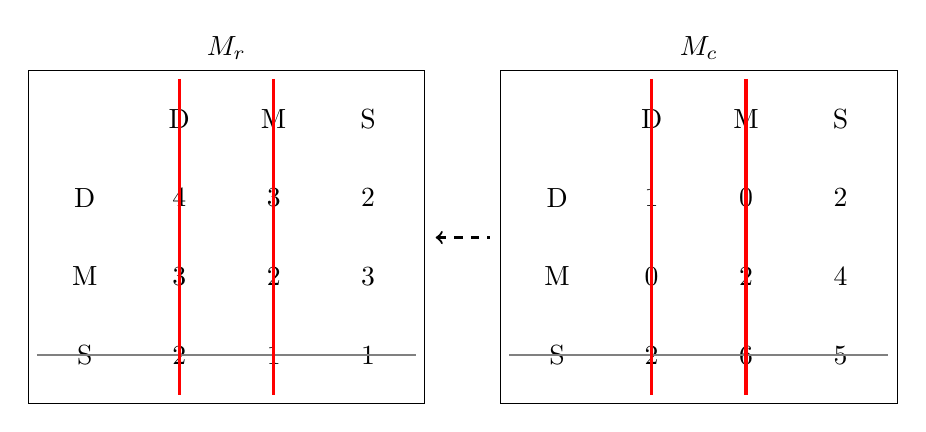
\begin{tikzpicture}
  \matrix (Mr1) [matrix of nodes, nodes={minimum width=1.2cm, minimum height=1cm, anchor=center},
    column sep=0pt, row sep=0pt, nodes in empty cells, draw=black, label=above:$M_r$] at (0,0)
  {
     & D & M & S \\
  D  & 4 & 3 & 2 \\
  M  & 3 & 2 & 3 \\
  S  & 2 & 1 & 1 \\
  };
  \draw[gray, thick] (Mr1-4-1.west) -- (Mr1-4-4.east);
  \draw[red, very thick] (Mr1-1-3.north) -- (Mr1-4-3.south);
  \draw[red, very thick] (Mr1-1-2.north) -- (Mr1-4-2.south);


  \matrix (Mc1) [matrix of nodes, nodes={minimum width=1.2cm, minimum height=1cm, anchor=center},
    column sep=0pt, row sep=0pt, nodes in empty cells, draw=black,
    label=above:$M_c$] at (6,0)
  {
     & D & M & S \\
  D  & 1 & 0 & 2 \\
  M  & 0 & 2 & 4 \\
  S  & 2 & 6 & 5 \\
  };
  \draw[gray, thick] (Mc1-4-1.west) -- (Mc1-4-4.east);
  \draw[red, very thick] (Mc1-1-3.north) -- (Mc1-4-3.south);
  \draw[red, very thick] (Mc1-1-2.north) -- (Mc1-4-2.south);

    \draw[black, <-, thick, dashed] ($(Mr1-2-4.south east) + (.25, 0)$) -- ($(Mc1-2-1.south west) +(-.25, 0) $);
\end{tikzpicture}
\end{document}
